%%%%%%%%%%%%%%%%%%%%%%%%%%%%%%%%%%%%%%%%%%%%%%%%%%%%%%%%%%%
%% Congratulations, you've made an excellent choice
%% of writing your Tampere University thesis using
%% the LaTeX system. This document attempts to be
%% as complete a template as possible to let you focus
%% on the most important part: the writing itself.
%% Thus the details regarding the visual appearance
%% and even structure have already been worked out
%% for you!
%%
%% I sincerely hope you will find this template useful
%% in completing your thesis project. I've tried to
%% add comments (followed by the % sign) to clarify
%% the structure and purpose of some of the commands.
%% Most of the magic happens in the file tauthesis.cls,
%% which you are more than welcome to take a look at.
%% Just refrain from editing it in the most crucial
%% versions of the thesis!
%%
%% I wish you and your thesis project the best of luck!
%% If this template causes you trouble along the way
%% or if you've any suggestions for improving it,
%% please be in contact through GitHub
%% (<URL HERE>)
%%
%% Yours,
%%
%% Ville Koljonen
%%
%% PS. This template or its associated class file don't
%% come with a warranty. The content is provided as is,
%% without even the implied promise of fitness to the
%% mentioned purpose. You, as the author of the thesis,
%% are responsible for the entire work, including the
%% provided material. No one else is liable to you for
%% any damage inflicted on you or your thesis, were it
%% caused by using this template or not.
%%%%%%%%%%%%%%%%%%%%%%%%%%%%%%%%%%%%%%%%%%%%%%%%%%%%%%%%%%%

%%%%% NOTICE %%%%%
%% Please read through the entire template
%% (files under ./tex) to find all instructions.
%% It is possible that the attached pdf files
%% do not include the latest information.
%%%%%%%%%%%%%%%%%%

%%%%% INSTRUCTIONS FOR COMPILING THE DOCUMENT %%%%%
%% Overleaf: just click Recompile.
%% Terminal:
%%  1. pdflatex main.tex
%%  2. makeindex -s main.ist -t main.glg -o main.gls main.glo
%%  3. biber main
%%  4. pdflatex main.tex
%%  5. pdflatex main.tex
%% Similar sequence of commands is also required
%% in LaTeX specific editors.
%%%%%%%%%%%%%%%%%%%%%%%%%%%%%%%%%%%%%%%%%%%%%%%%%%%

%%% Set PDF version before doing anything else.

\input{set-pdf-version.tex}

%%%%% METADATA %%%%%
%
% Always keep the following metadata up to date! This is important for your
% PDF file to comply to accessibility standards. (And yes, this information
% must remain here, before \documentclass[...]{...}.)

\def\myfititle{Dieselmoottorin hiukkassuodattimen tilan estimointi}
\def\myentitle{State Estimation of a Diesel Particulate Filter}
\def\myauthor{Tuomas Haataja}
\def\myfisubtitle{}
\def\myensubtitle{}
\def\myfithesistype{Diplomityö}
\def\myenthesistype{Masters of Science Thesis}
\def\myexaminers{Veli-Pekka Pyrhönen \\ Prof. Matti Vilkko}
\def\myfifacultyname{Tekniikan ja luonnontieteiden tiedekunta}
\def\myenfacultyname{Faculty of Engineering and Natural Sciences}
\def\myfiprogrammename{Automaatiotekniikka}
\def\myenprogrammename{Automation Engineering}
\def\myfikeywords{Hiukkassuodatin, DPF, noki}
\def\myenkeywords{Diesel Particulate Filter, DPF, soot}
\def\mylanguagecode{en-GB}
\def\mysubject{A short description of the thesis subject.}
\def\myyear{2025}
\def\mymonth{08}
\def\myday{31}

% Define your citation options here. Valid values for style and sorting options
% can be found in the BibLaTeX manual: https://ctan.org/pkg/biblatex.

\def\mycitationstyle{numeric}
%\def\mycitationsorting{nyt}
\def\mycitationsorting{none}

%%%%% PREAMBLE %%%%%

%%%%% Document class declaration.
%
% The possible optional arguments are
%
%   finnish - thesis in Finnish (default)
%   english - thesis in English
%   draft - for faster non-final works, also skips images
%           (recommended, remove in final version)
%   programs - if you wish to display code snippets
% Example: \documentclass[english, authoryear]{tauthesis}
%          thesis in English with author-year citations

\documentclass[finnish]{tauthesis}

\input{preamble.tex} % You can add packages and define new commands in this file.
\newcommand{\doo}{\partial}

%\makeglossaries
\begin{document}

%%%%% FRONT MATTER %%%%%

\frontmatter

%%%%% Thesis information and title page.

\input{titlepage.tex}

%%%%% Abstracts and preface.
%
% Write the abstract(s) and the preface into a separate file for the sake of
% clarity. Pass the appropriate file name as the first argument to these
% commands. Put the \abstract in the primary language first and the
% \otherabstract in the secondary language second. Those who do not speak
% Finnish only need the first abstract. The second argument of the \preface
% command takes the place where the thesis was signed in.
%
% Edit the files tex/{use-of-ai,tekoalyn-kaytto}.tex to match your use of AI in
% generating this thesis.
%

\abstract{tex/tiivistelma.tex}

\otherabstract{tex/abstract.tex}

\aidisclaimerinclusioncmd

\preface{tex/alkusanat.tex}{Tampereella}

%%%%% Table of contents.

\tableofcontents

%%%%% Lists of figures, tables, listings and terms.
%
% Print the lists of figures and/or tables. Uncomment either of these commands
% as required. Both are optional, but if there are many important
% figures/tables, listing them may be a good idea.

% \listoffigures
% \listoftables
% \lstlistoflistings

% Misc stuff related to how the glossary is displayed. You can especially
% tweak the lengths to suit you!

\glsaddall
\setglossarystyle{taulong}
\setlength{\glsnamewidth}{0.25\textwidth}
\setlength{\glsdescwidth}{0.75\textwidth}
\renewcommand*{\glsgroupskip}{}

% Print the default glossary of abbreviations, if necessary. Otherwise comment
% out. The appropriate Finnish variant is 'Lyhenteet'

\printglossary[title={Lyhenteet ja merkinnät}]

%\printglossaries
% Print more than one glossary with these lines. Otherwise comment out.

% \printglossary[type=symbs]
% \printglossary[type=label]
% ...

%%%%% MAIN MATTER %%%%%

\mainmatter

% Write each of the chapters of the thesis into a separate file for the sake
% of clarity. They can be \input as shown below. Give both the chapters and
% their files as descriptive names as possible.

\chapter{Johdanto}%
\label{ch:johdanto}
Dieselmoottori on muun muassa toimintavarmuutensa ja energiatehokkuutensa vuoksi yksi nykypäivän merkittävimmistä voimanlähteistä.  
\cite[s. 121, 137-138]{Koten_2024}.
Pelkästään Yhdysvalloissa noin 75\% maatalouden työkoneista käyttää dieselmoottoria voimanlähteenään \cite[s. 122]{Koten_2024}.  
Dieselmoottori kuitenkin tuottaa palamisolosuhteiden vuoksi
huomattavasti päästöjä \cite{FiebigMichael2014Pefd}. Erityisesti typen oksidi- (NO\(_x\)) ja hiukkaspäästöt (PM) ovat ongelma niin terveydelle kuin ympäristöllekin \cite{FiebigMichael2014Pefd}\cite[s. 138]{Koten_2024}, joten  lainsäädäntö asettaa yhä tiukentuvat rajat dieselmoottorien päästöille. Tämän vuoksi moderneissa työkoneissa on käytettävä pakokaasun jälkikäsittelyjärjestelmiä, jotka pyrkivät minimoimaan dieselmoottorin tuottamien haitallisten päästöjen pääsyä ilmakehään. Koska lainsäädännön rajat tiukentuvat, täytyy kehittää ja parantaa jatkuvasti.

Hiukkaspäästöjä voidaan pienentää merkittävästi hiukkassuodattimella (DPF, \emph{eng. Diesel Particulate Filter}). DPF suodattaa läpi virtaavasta pakokaasusta jopa 99\% hiukkaslukumäärästä ja 95\% -massasta \cite{Yan_state_of_the_art}.


\chapter{Hiukkassuodatin}%
\label{ch:dpf}


Dieselmoottorin hiukkassuodatin, eli DPF (\emph{eng. Diesel Particulate Filter}) on tehokkain järjestelmä pakokaasun noki- ja tuhkapartikkeleiden suodatukseen. 
Hyvä DPF suodattaa läpivirtaavasta pakokaasusta jopa 99\% hiukkaslukumäärästä ja 95\% -massasta \cite{Yan_state_of_the_art}. 

\begin{figure}[H]
    \centering
    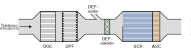
\includegraphics[width=\textwidth]{figures/EAT.pdf}
\end{figure}

\section{Järjestelmän fyysinen rakenne}

Tyypillisin DPF-tyyppi on ns. seimämävirtaus-DPF (\emph{eng. wall-flow DPF}), jossa pakokaasu virtaa vuoronperään vastakkaisista päistään suljetuissa putkissa. Pakokaasu virtaa putkien välillä huokoisten seinämien läpi. Virtausta on havainnollistettu Kuvassa \ref{fig:wall-flow-dpf}  


\begin{figure}[H]
    \centering 
    
    \pdftooltip{
\begin{tikzpicture}[scale=2]
    % Drawing gray squares between the lines
    \fill[gray] (0, 0) rectangle (0.5, 0.5);  
    \fill[gray] (0, 1.0) rectangle (0.5, 1.5); 
    \fill[gray] (4.5, 0.5) rectangle (5, 1.0); 
    \fill[gray] (4.5, 1.5) rectangle (5, 2.0); 
    
    % Drawing 5 parallel horizontal lines with 0.5 unit spacing
    \foreach \y in {0, 0.5, 1, 1.5, 2} {
        \draw[line width=3pt, black]  (0, \y) -- (5, \y);
    }
    % For widening the lines
    % \draw[line width=3pt, black]  (0, -0.05) -- (5, -0.05);
    % \draw[line width=3pt, black]  (0, 2.05) -- (5, 2.05);

    % Adding arrows pointing to the gaps with no squares
    \draw[-{Latex}, thick, red] (-1, 0.75) -- (-0.1, 0.75);
    \draw[-{Latex}, thick, red] (-1, 1.75) -- (-0.1, 1.75); 
    \draw[-{Latex}, thick, red] (5.1, 0.25) -- (6, 0.25); 
    \draw[-{Latex}, thick, red] (5, 1.25) -- (6, 1.25); 

   \draw[-{Latex}, thick, red] (0.5, 0.75) to[out=0, in=180] (1.5, 0.25);
    \draw[-{Latex}, thick, red] (0.5, 0.75) to[out=0, in=180] (1.5, 1.25);
    \draw[-{Latex}, thick, red] (2.5, 0.75) to[out=0, in=180] (3.5, 0.25);
    \draw[-{Latex}, thick, red] (2.5, 0.75) to[out=0, in=180] (3.5, 1.25);
    
    
    
    \draw[-{Latex}, thick, red] (1.5, 1.75) to[out=0, in=180] (2.5, 1.25);
    \draw[-{Latex}, thick, red] (3.5, 1.75) to[out=0, in=180] (4.5, 1.25);
\end{tikzpicture}

}
                {Kuvituskuvassa on neljä päällekkäistä putkea. Nuolilla kuvattu pakokaasu virtaa vasemmalta avoimiin putkiin. Putket ovat suljettuja oikeasta päästään, joten nuolet kulkevat putkien välisen seinämän läpi putkiin, jotka ovat avoimia oikealta. Nuolet poistuvat putkista oikealta puolelta.
                }
    \caption{Pakokaasu virtaa suodattimessa huokoisten seinämien läpi. Yli 90\% pakokaasun hiukkasmassasta jää huokoisten seinämien sisään ja pinnalle.}
    \label{fig:wall-flow-dpf}
\end{figure}



\section{Regenerointi}
\begin{align*}
    \ce{C + 1/2 O2 &-> CO }\\
    \ce{C + O2 &-> CO2}\\
    \ce{C + NO2 &-> CO +  NO}  \\
    \ce{C + 2 NO2 &-> CO2 + 2 NO}  \\
    \ce{C + NO2 + 1/2 O2 &-> CO2 + NO}  \\
    \ce{C + NO2 + 1/2 O2 &-> CO + NO2} 
\end{align*}


\section{Hiukkassuodattimen matemaattinen esitys}

\begin{figure}[H]
    \centering 
    \begin{tikzpicture}
    % Draw the first rectangle
    \node[draw, rectangle, minimum width=1.5cm, minimum height=3cm] (rect1) at (0, 0) {Rectangle 1};

    % Draw the second rectangle
    \node[draw, rectangle, minimum width=1.5cm, minimum height=3cm] (rect2) at (4, 0) {Rectangle 2};

    % Draw arrows between rectangles
    \draw[-{Latex}, thick] ([yshift=-0.5cm]rect1.north east) -- ([yshift=-0.5cm]rect2.north west);
    \draw[-{Latex}, thick] ([yshift=0.5cm]rect1.south east) -- ([yshift=0.5cm]rect2.south west);

    % Draw inputs to rect1
    \draw[-{Latex}, thick] (-3, 1) -- ([yshift=1cm]rect1.west) node[above left] {Nokilataus (g/l)};
    \draw[-{Latex}, thick] (-3, -1) -- ([yshift=-1cm]rect1.west) node[below left] {Tuhkalataus (g/l)};

    % Draw output from rect2
    \draw[-{Latex}, thick] (rect2.east) -- (7, 0) node[above right] {Paine (hPa)};

\end{tikzpicture}
    \caption{}
    \label{fig:blocks1}
\end{figure}
\cite{LiuGuanlin2021Roio}


\chapter{Systeemin tilan estimointi }%Bayesilaisilla suotimilla}%
\label{ch:estimointi}
Optimaaliset suotimet ovat  matemaattisia menetelmiä, joilla estimoidaan systeemien tiloja kohinaisiin mittauksiin perustuen \cite{sarkka_bayesian}. Tässä työssä tarkastellaan Bayesilaisia suotimia, jotka ratkaisevat optimointiongelman Bayesilaisittain. 

\section{Teoreettista taustaa}
{\color{red} (nimi vaihtuu), Lyapunov ja Riccati yms.}

\section{Kalman-suodin}

Kalman-suodin on algoritmi, jolla voidaan estimoida lineaarisen ja kohinaisen systeemin tilaa. Systeemin kohinan tulee olla valkoista kohinaa \cite[s. 56]{sarkka_bayesian}. Algoritmi on kaksivaiheinen ja se koostuu ennuste- ja päivitysvaiheista. 
Ennustevaihe tehdään lähtökohtaisesti jokaisella aika-askeleella. Päivitysvaihe sen sijaan voidaan laskennan tai saavuttamattoman mittauksen vuoksi toteuttaa harvemminkin. 

Tarkastellaan lineaarista systeemiä
\begin{align}
    \begin{split}
        x_k &= A_{k-1}x_{k-1} + w_{k-1} \\
        y_k &= H_k x_k + v_k,
    \end{split}
\end{align}
jossa \(x_k \in \R^n \) on systeemin tila hetkellä \(k\), \(A_{k-1}\in \R^{n\times n}\) on tilamatriisi, \(y_k\in \R^m\) on mittaus, \(H_k \in \R^{m \times n}\) on mittausmatriisi. Muuttujat \(w_{k-1} \sim \mathcal{N}(0, Q_{k-1})\) ja \(v_k \sim \mathcal{N}(0, R_k)\) ovat normaalijakautuneet (Gaussiset) prosessi- ja mittauskohinat, joissa \(Q_{k-1}\) ja \(R_k\) ovat vastaavat kovarianssimatriisit. Tilan ja mittauksen estimaatteja merkitään \(\hat{x}_k\) ja \(\hat{y}_k\).

Kalman-suodin ratkaisee jokaisella iteraatiolla normaalijakautuneen estimaatin, jossa keskiarvo on \(\hat{x}_k\) ja optimoitu kovarianssi on \(P_k\).  

Ennustevaihe:
\begin{align}
    \hat{x}_{k | k-1}  &= A_{k-1} \hat{x}_{k-1}\\
    P_{k | k-1} &= A_{k-1} P_{k-1} A_{k-1}^T + Q_{k-1}.
\end{align}

Päivitysvaihetta varten tarvitaan mittausennuste
\begin{align}
    \hat{y}_k = H_k \hat{x}_{k | k-1} 
\end{align}
ja Kalman-vahvistus 
\begin{align}
    K_k = P_{k | k-1} H_k^T \left(H_k P_{k | k-1} H_k^T + R_k \right)^{-1}.
\end{align}
Kalman-vahvistuksen yhtälö minimoi todellisen ja estimoidun tilan keskiarvon neliöllisen virheen \cite{sparse_kalman_gain}, ja se määrittää kuinka paljon uuteen mittaukseen uskotaan vanhaan estimaattiin verrattuna \cite{becker2023kalman}.

Päivitysvaihe:
\begin{align}
    \hat{x}_{k | k} &= \hat{x}_{k | k-1} + K_k (y_k - \hat{y}_k)\\
    P_{k|k}         &= (I - K_k H_k)P_{k|k-1},
\end{align}
jossa \(I \in \R^{n\times n}\) on identiteettimatriisi.

\section{EKF}
Toisin kuin tavallinen Kalman-suodin, laajennettu Kalman-suodin, eli EKF \emph{(eng. Extended Kalman Filter)} kykenee ratkaisemaan epälineaaristen funktioiden optimointiongelman lähes optimaalisesti. Menetelmä perustuu funktioiden linearisointiin, joten ratkaisu ei välttämättä ole täysin optimaalinen, mutta usein riittävän optimaalinen. Menetelmä kuitenkin vaatii funktioiden derivoituvuutta, sillä algoritmissa ratkaistaan sekö tilanfunktion että mittausfunktion Jacobin matriisit joka iteraatiolla. Tarkastellaan diskreettiä systeemiä, jonka tilanyhtälö on
\begin{align}
    x_k = f(x_{k-1}, u_{k-1}) + w_{k-1},
\end{align}
ja mittausyhtälö on
\begin{align}
    z_k = h(x_{k}, u_{k}) + v_k.
\end{align}
Funktiot \(f\) ja \(h\) ovat yleisesti epälineaarisia ja derivoituvia. Prosessi- ja mittaushäiriöt \(w\) ja \(v\) ovat nollakeskiarvoisia ja normaalijakautuneita, ja niiden kovarianssimatriiseita merkitään \(Q\) ja \(R\).

Kuten tavallisellakin Kalman-suotimella, EKF-algoritmi voidaan jakaa ennuste- ja päivitysvaiheisiin. 
Ennustevaiheessa ratkaistaan uusi estimaatti sekä sen kovarianssimatriisi. Ennustevaihe on muotoa
\begin{align}
    \hat{x}_{k|k-1} &= f(\hat{x}_{k-1|k-1}, u_{k-1}) \\
    P_{k|k-1} &= F_k P_{k-1|k-1} F_k^T + Q_{k-1},
\end{align}
jossa \(F\) on funktion \(f\) Jacobin matriisi. 
Päivitysvaiheessa tilan päivitystä varten ratkaistaan Kalman-vahvistus
\begin{align}
    S_k &= H_k P_{k|k-1} H_k^T + R_k \\
    K_k &= P_{k|k-1} H_k^T S_k^{-1},
\end{align}
jossa \(H\) on funktion \(h\) Jacobin matriisi. 
Kalman-vahvistuksella ja mittauksen ja mallin välisellä virheellä  \(e_{z, k} = z_k - h(\hat{x}_{k|k-1}) \) 
voidaan päivittää estimaatti ja sen kovarianssi
\begin{align}
    \hat{x}_{k|k} &= \hat{x}_{k|k-1} + K_k e_{z, k}, \\
    P_{k|k} &= (I-K_k H_k) P_{k|k-1}.
\end{align}
Kalman-vahvistuksen epäoptimaalisuus johtuu linearisointien epätarkkuudesta. Täten EKF ei ole luotettava estimointialgoritmi pitkille aikaikkunoille, hitaille näytteenottotaajuuksille tai huonosti derivoituville funktioille.

\chapter{Hiukkassuodattimen tilan estimointi}%
\label{ch:dpf_estimointi}


Tässä luvussa laaditaan EFK-estimointialgoritmi noki-, ja tuhkalatauksille. Algoritmin tilanyhtälöt ovat \eqref{eq:tilanyhtalo_noki} ja \(\dot{m}_{ash} =\dot{m}_{ash,in}\), ja mittausyhtälö on \eqref{eq:deltaP_total}. 
Esitellään EKF-algoritmin muuttujat
\begin{align*}
    x &= \bm{m_{soot} \\ m_{ash}},  
    \qquad  u = \bm{ \dot{m}_{soot, in} \\ \dot{m}_{ash,in} \\ c_{NO_2, in}} 
    \\
    z &= \Delta P_{meas},
    \qquad \hat{z} =  \Delta P_{tot} \\
\end{align*}
Lämpötila tunnetaan tarkasti, joten se voidaan jättää mallin parametriksi. Hapen konsentraatio on useita kertaluokkia korkeampi kuin typpidioksidin, joten sitä ei tarvita sisäänmenoksi. 
EKF-algoritmia voidaan käyttää, kunhan funktiot linearisoidaan. 
Painehäviömallin funktiot ovat derivoituvia kaikkialla, joten painehäviöyhtälöt voidaan linearisoida.
Linearisointi on toteutettu liitteessä \ref{ch:dP_linearisointi}.

\chapter{Tulokset}%
\label{ch:tulokset}

\chapter{Yhteenveto}%
\label{ch:yhteenveto}





%%%%% Bibliography/references.

% Print the bibliography according to the information in ./tex/references.bib
% and the in-line citations used in the body of the thesis.

% \emergencystretch=2em
\printbibliography[heading=bibintoc]

%%%%% Appendices.

% Use only if it clarifies the structure of the document. Remember to
% introduce each appendix and its content.

\begin{appendices}


\chapter{Painehäviömallin linearisointi}%
\label{ch:linearisointi}

Tässä liitteessä johdetaan painehäviömallin yhtälöiden linearisointi. Yleisesti linearisointi kohdassa \(x_0\) voidaan esittää muodossa
\begin{align}
    \tilde{f}(x) = f(x_0) \sum_{k=1}^n \frac{\doo f(x_0)}{\doo x_k} (x_k-x_0),
\end{align}
jossa \(x, x_0 \in \R^k\). 
Painehäviöt \(\Delta P_{inlet}\), \(\Delta P_{ash}\) ja \(\Delta P_{soot}\) riippuvat noki- ja tuhkakerroksista \(w_{soot}\) ja \(w_{ash}\). 
Linearisointi toteutetaan muuttujien \(m_{soot}\) ja \( m_{ash}\) suhteen, joten
sovelletaan derivoinnin ketjusääntöä
\begin{align}
    \nabla (f \circ g)(x) = \nabla f(g(x))\nabla g(x).
\end{align}
Linearisoidaan  yhtälöt \eqref{eq:deltaP_inlet}--\eqref{eq:deltaP_soot}.


% Tuhkakerroksen paksuuden linearisointi on 
% \begin{align}
%     \tilde{w}_{ash}( m_{soot},  m_{ash}) = \frac{\doo w_{ash}}{\doo m_{soot}}  \Delta m_{soot}
%                                                     + \frac{\doo w_{ash}}{\doo m_{ash}} \Delta m_{ash},
% \end{align} 
% ja nokikerroksen 
% \begin{align}
%     \tilde{w}_{soot}( m_{soot},  m_{ash}) = \frac{\doo w_{soot}}{\doo m_{soot}}  \Delta m_{soot}
%                                                     + \frac{\doo w_{soot}}{\doo m_{ash}} \Delta m_{ash}.
% \end{align}
% Yhtälö ei riipu noen määrästä, joten
% \begin{align}
%     \tilde{w}_{ash}( m_{soot},  m_{ash}) =  \frac{\Delta m_{ash}}
%     {4L n_{open} \rho_{ash}\sqrt{\alpha_{in}^2 - \frac{m_{ash, 0}}{L n_{open} \rho_{ash}}}}.
% \end{align}

% Nokikerroksen paksuuteen vaikuttaa myös tuhkakerroksen paksuus. Sijoittamalla yhtälö \eqref{eq:deltaP_wash} yhtälöön \eqref{eq:deltaP_wsoot}, saadaan
% \begin{align}
%     w_{soot}(m_{soot}, m_{ash}) =
%     \frac{ \sqrt{\alpha_{in}^2 - \frac{m_{ash}}{L n_{open} \rho_{ash}}}
%             - 
%            \sqrt{\alpha_{in}^2 - \frac{m_{ash}}{L n_{open} \rho_{ash}} - \frac{m_{soot}}{L n_{open} \rho_{soot}}} }
%     {2}.
% \end{align}

% \begin{align}
%     \begin{split}
%     \tilde{w}_{soot}(m_{soot}, m_{ash}) = &
%     \frac{\Delta m_{soot}}{4 L n_{open} \rho_{{soot}} \sqrt{a_{{in}}^2 - \frac{m_{{ash,0}}}{L n_{open} \rho_{{ash}}} - \frac{m_{{soot,0}}}{L n_{open} \rho_{{soot}}}}} + \\
%     & \frac{\Delta m_{ash}}{4 L n_{open} \rho_{{ash}} \sqrt{a_{{in}}^2 - \frac{m_{{ash,0}}}{L n_{open} \rho_{{ash}}} - \frac{m_{{soot,0}}}{L n_{open} \rho_{{soot}}}}} - \\ &
%     \frac{\Delta m_{ash}}{4 L n_{open} \rho_{{ash}} \sqrt{a_{{in}}^2 - \frac{m_{{ash,0}}}{L n_{open} \rho_{{ash,0}}}}}
%     \end{split}
% \end{align}

% Paremmin näin
Ratkaistaan noki- ja tuhkakerrosten derivaatat noen ja tuhkan suhteen derivoimalla yhtälöt \eqref{eq:deltaP_ash} ja \eqref{eq:deltaP_soot}.
Esitellään apumuuttujat
\begin{align*}
    a &:= L n_{open}, \\
    b &:= \sqrt{\alpha_{in}^2 - \frac{m_{ash}}{L n_{open} \rho_{ash}}}, \\
    c &:= \sqrt{\alpha_{in}^2 - \frac{m_{ash}}{L n_{open} \rho_{ash}} - \frac{m_{soot}}{L n_{open} \rho_{soot}}}.
\end{align*}

Tuhkakerroksen derivaatat ovat
\begin{align}
    \frac{\doo w_{ash}}{\doo m_{soot}} & =0\\
    \frac{\doo w_{ash}}{\doo m_{ash}} &= \frac{1}{ab\rho_{ash}},
\end{align}
ja vastaavasti nokikerroksen derivaatat ovat
\begin{align}
    \frac{\doo w_{soot}}{\doo m_{soot}} &= \frac{1}{ac\rho_{soot}}\\
    \begin{split}
    \frac{\doo w_{soot}}{\doo m_{ash}} &= \frac{1}{ac\rho_{ash}}-\frac{1}{ab\rho_{ash}}
    \\ &= \frac{ab \rho_{ash} - ac\rho_{ash}}{ab\rho_{ash}\cdot ac \rho_{ash}}
    \\ &= \frac{\cancel{a}\cancel{\rho_{ash}}(b-c)}{a^{\cancel{2}} \rho_{ash}^{\cancel{2}} bc}
    \\ &= \frac{b-c}{abc\rho_{ash}}
    \end{split}
\end{align}
Laaditaan derivaatoista Jacobin matriisi
\begin{align}
    J_m(m_{soot}, m_{ash}) = 
    \bm{
        \frac{\doo w_{soot}}{\doo m_{soot}} & \frac{\doo w_{soot}}{\doo m_{ash}}
    \\  \frac{\doo w_{ash}}{\doo m_{soot}} & \frac{\doo w_{ash}}{\doo m_{ash}}
    }.
\end{align}

% Tuhkakerroksen paksuuden linearisointi saadaan muotoon
% \begin{align}
%     \tilde{w}_{ash}( m_{soot},  m_{ash}) =
%     \frac{1}{ \rho_{ash} \, ab}\Delta m_{ash}.
% \end{align}

% % \begin{align}
% %     w_{soot}(m_{soot}, m_{ash}) =
% %     \frac{b - c}{2}.
% % \end{align}

% \begin{align}
% \begin{split}
%     \tilde{w}_{soot}(m_{soot}, m_{ash}) = 
%     \frac{1}{  ac \rho_{{soot}} } \Delta m_{soot} +
%     \frac{b-c}{abc\rho_{{ash}} } \Delta m_{ash} 
% \end{split}
% \end{align}




Derivoidaan yhtälö \eqref{eq:deltaP_total}. Saadaan
\begin{align}
    \nabla \Delta P_{tot}(m_{soot}, m_{ash})=
    \bm{  \frac{\doo \Delta P_{tot}}{\doo w_{soot}}
        &   \frac{\doo \Delta P_{tot}}{\doo w_{ash}}
        }
    \bm{
        \frac{\doo w_{soot}}{\doo m_{soot}} & \frac{\doo w_{soot}}{\doo m_{ash}}
    \\  \frac{\doo w_{ash}}{\doo m_{soot}} & \frac{\doo w_{ash}}{\doo m_{ash}}
        }
\end{align}
Linearisointiin tarvittavat derivaatat ovat 
\begin{align}
    \frac{\doo \Delta P_{tot}}{\doo m_{soot}} &=
        \frac{\doo w_{soot}}{\doo m_{soot}}
        \frac{\doo \Delta P_{tot}}{\doo w_{soot}}
        +
        \frac{\doo w_{ash}}{\doo m_{soot}}
        \frac{\doo \Delta P_{tot}}{\doo w_{ash}}
    \\
    \frac{\doo \Delta P_{tot}}{\doo m_{ash}} &=
        \frac{\doo w_{soot}}{\doo m_{ash}}
        \frac{\doo \Delta P_{tot}}{\doo w_{soot}}
        +
        \frac{\doo w_{ash}}{\doo m_{ash}}
        \frac{\doo \Delta P_{tot}}{\doo w_{ash}}.
\end{align}

Linearisointi on muotoa
\begin{align}
    \begin{split}
    \Delta\tilde{ P}_{tot}(m_{soot, 0}, m_{ash, 0}) &= \Delta P_{tot}(m_{soot, 0}, m_{ash, 0})
    \\ &+
    \frac{\doo {\Delta P}_{tot}(m_{soot, 0}, m_{ash, 0})}{\doo m_{soot}} (m_{soot} - m_{soot,0}) 
    \\ &+ 
    \frac{\doo {\Delta P}_{tot}(m_{soot, 0}, m_{ash, 0})}{\doo m_{ash}}  (m_{ash} - m_{ash,0})
    \end{split}
\end{align}



\end{appendices}

\end{document}
